\documentclass[12pt]{report}

\usepackage[utf8]{inputenc}
\usepackage{graphicx}
\usepackage{geometry}
\usepackage{hyperref}
\usepackage{setspace}
\usepackage{fancyhdr}
\usepackage{multicol}
\usepackage{titlesec}
\hypersetup{
    colorlinks=true,
    linkcolor=black,      
    urlcolor=blue,
}
\titlespacing*{\chapter}{0pt}{0pt}{*}
\geometry{
 a4paper,
 top=15mm
}

\begin{document}
\begin{titlepage}
    \centering
    \vspace*{1cm}

    {\Huge Indian Institute of Technology, Dharwad} \\
    \vspace{1cm}
    \includegraphics[width=0.35\textwidth]{IIT_Dharwad_Emblem_white.png} \\
    \vspace*{1cm}
    {\Huge CS 209/214 - Artificial Intelligence \\
    Term Project Report \par}
    \vspace{1.5cm}

    \Large{
    \textbf{Course Instructor:}\\
    Dr. Dileep A. D.\\
    \vspace{1cm}
    \textbf{Mentor:}\\
    Ms. Neha Rudrappa Pudakalakatti\\}
    \vfill
    {\LARGE Team 21 \par}
    \vspace{1cm}
    {\large
    \begin{tabular}{ll}
    Raghuveer Verma & \hspace{1cm} \textsf{CS23BT041} \\
    Annavarapu Vijwal & \hspace{1cm} \textsf{MC23BT001} \\
    Shaikh Aariz & \hspace{1cm} \textsf{MC23BT030} \\
    Abhinandan Jain & \hspace{1cm} \textsf{CS23BT012} \\
    \end{tabular}
    }
    
\end{titlepage}

\newpage
\begin{center}
    \textbf{Abstract}
\end{center}
In this project, we explore and compare various Machine Learning models for three tasks: Classification, Regression, and Clustering. The data set used contains features that describe the financial situation and personal attributes of individuals.

In classification, the goal is to predict whether a loan is approved or not. For the regression task, we use models to estimate an individual's risk score. Clustering involves identifying clusters in the data, where we use techniques such as the Elbow Method and Silhouette Analysis to get the optimal number of clusters.

\pagenumbering{roman}
\tableofcontents
\newpage

\pagenumbering{arabic}
\setcounter{page}{1}

\chapter{The Dataset}
% \addcontentsline{toc}{chapter}{The Dataset}
We use a synthetic dataset comprising of 20,000 records of personal and financial data. The original dataset can be found \href{https://www.kaggle.com/datasets/lorenzozoppelletto/financial-risk-for-loan-approval?select=Loan.csv}{here}.

\phantomsection
\section*{Features}
\addcontentsline{toc}{section}{Features}
The dataset contains the following thirty-six columns:
\begin{multicols}{2}
\begin{enumerate}
    \item Demographic and \\ Employment Information
    \begin{itemize}
        \item Age
        \item Marital Status
        \item Number of Dependents
        \item Education Level
        \item Employment Status
        \item Experience
        \item Job Tenure
    \end{itemize}
    \item Financial and Credit Information
    \begin{itemize}
        \item Annual Income
        \item Monthly Income
        \item Total Assets
        \item Total Liabilities
        \item Net Worth
        \item Home Ownership Status
        \item Savings Account Balance
        \item Checking Account Balance
        \item Debt-to-Income Ratio
        \item Total Debt-to-Income Ratio
        \item Monthly Debt Payments
        \item Utility Bills Payment History
    \end{itemize}
    \item Credit History and \\ Loan Information
    \begin{itemize}
        \item Credit Score
        \item Credit Card Utilization Rate
        \item Number of Open Credit Lines
        \item Number of Credit Inquiries
        \item Bankruptcy History
        \item Length of Credit History
        \item Previous Loan Defaults
        \item Payment History
    \end{itemize}
    \item Loan Attributes
    \begin{itemize}
        \item Loan Amount
        \item Loan Duration
        \item Loan Purpose
        \item Base Interest Rate
        \item Interest Rate
        \item Monthly Loan Payment
        \item Application Date
    \end{itemize}
    \item Target Variables
    \begin{itemize}
        \item Loan Approved
        \item Risk Score
    \end{itemize}
\end{enumerate}
\end{multicols}

\phantomsection
\addcontentsline{toc}{section}{Analysis and Preprocessing}
\section*{Analysis and Preprocessing}

\phantomsection
\addcontentsline{toc}{subsection}{Duplicate and Missing Values}
\textbf{Duplicate and Missing Values:}
No duplicate rows or rows with missing values were found.
\\ \\

\phantomsection
\addcontentsline{toc}{subsection}{Columns with Multiple Classes}
\noindent\textbf{Columns with multiple classes:}
The following columns described multiple classes as strings which were later converted to integer labels (given on the left) and one-hot encodings in separate datasets:
\begin{itemize}
    \item \textbf{Employment Status}
    \begin{itemize}
        \item 0: Employed
        \item 1: Self-Employed
        \item 2: Unemployed
    \end{itemize}
    \item \textbf{Education Level}
    \begin{itemize}
        \item 0: Master
        \item 1: Associate
        \item 2: Bachelor
        \item 3: High School
        \item 4: Doctorate
    \end{itemize}
    \item \textbf{Marital Status}
    \begin{itemize}
        \item 0: Married
        \item 1: Single
        \item 2: Divorced
        \item 3: Widowed
    \end{itemize}
    \item \textbf{Home Ownership Status}
    \begin{itemize}
        \item 0: Own
        \item 1: Mortgage
        \item 2: Rent
        \item 3: Other
    \end{itemize}
    \item \textbf{Loan Purpose}
    \begin{itemize}
        \item 0: Home
        \item 1: Debt Consolidation
        \item 2: Education
        \item 3: Other
        \item 4: Auto
    \end{itemize}
\end{itemize}

\newpage
\noindent
\phantomsection
\addcontentsline{toc}{subsection}{Visualizations}
\textbf{Visualizations}
\\

\null
\vspace*{\fill}
\noindent\makebox[\textwidth]{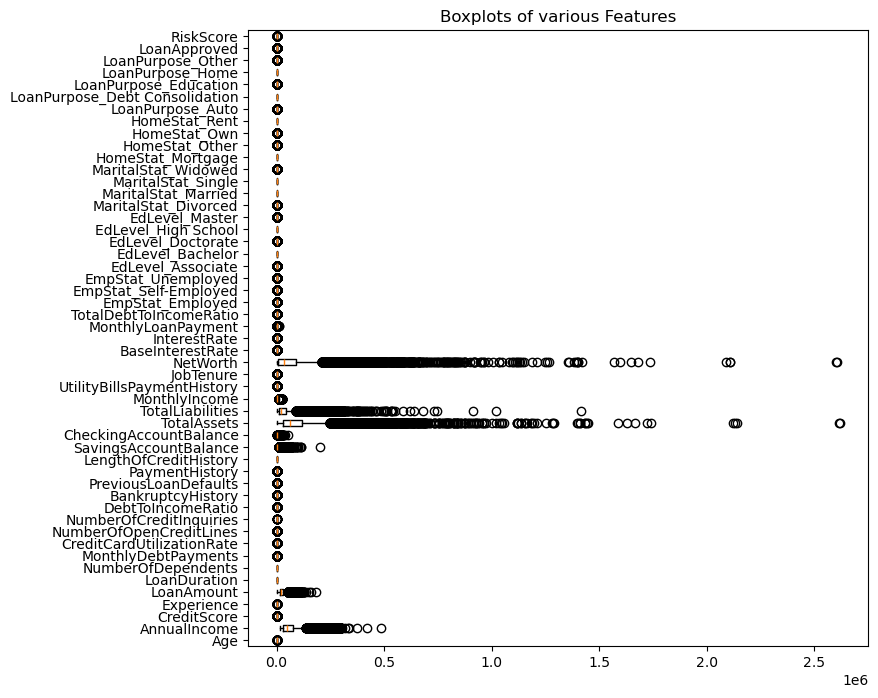
\includegraphics[width=0.9\paperwidth]{boxplot.png}}
\label{boxplot}
\vspace*{\fill}

\newpage
\null
\vspace*{\fill}
\noindent\makebox[\textwidth]{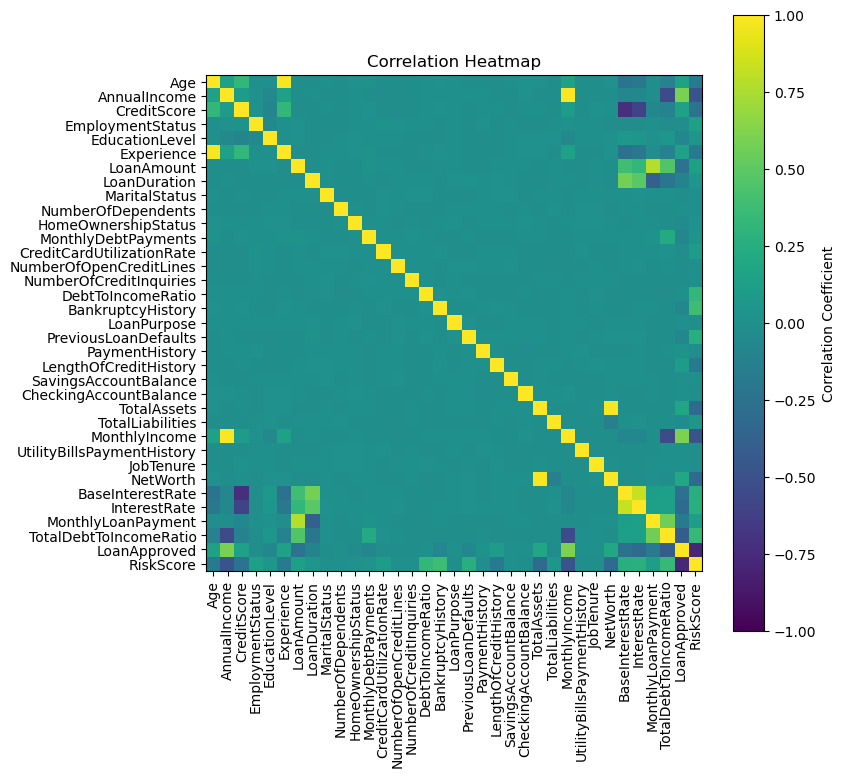
\includegraphics[width=0.9\paperwidth]{CorrHeatMap.png}}
\vspace*{\fill}

\newpage
\null
\vspace*{\fill}
\noindent\makebox[\textwidth]{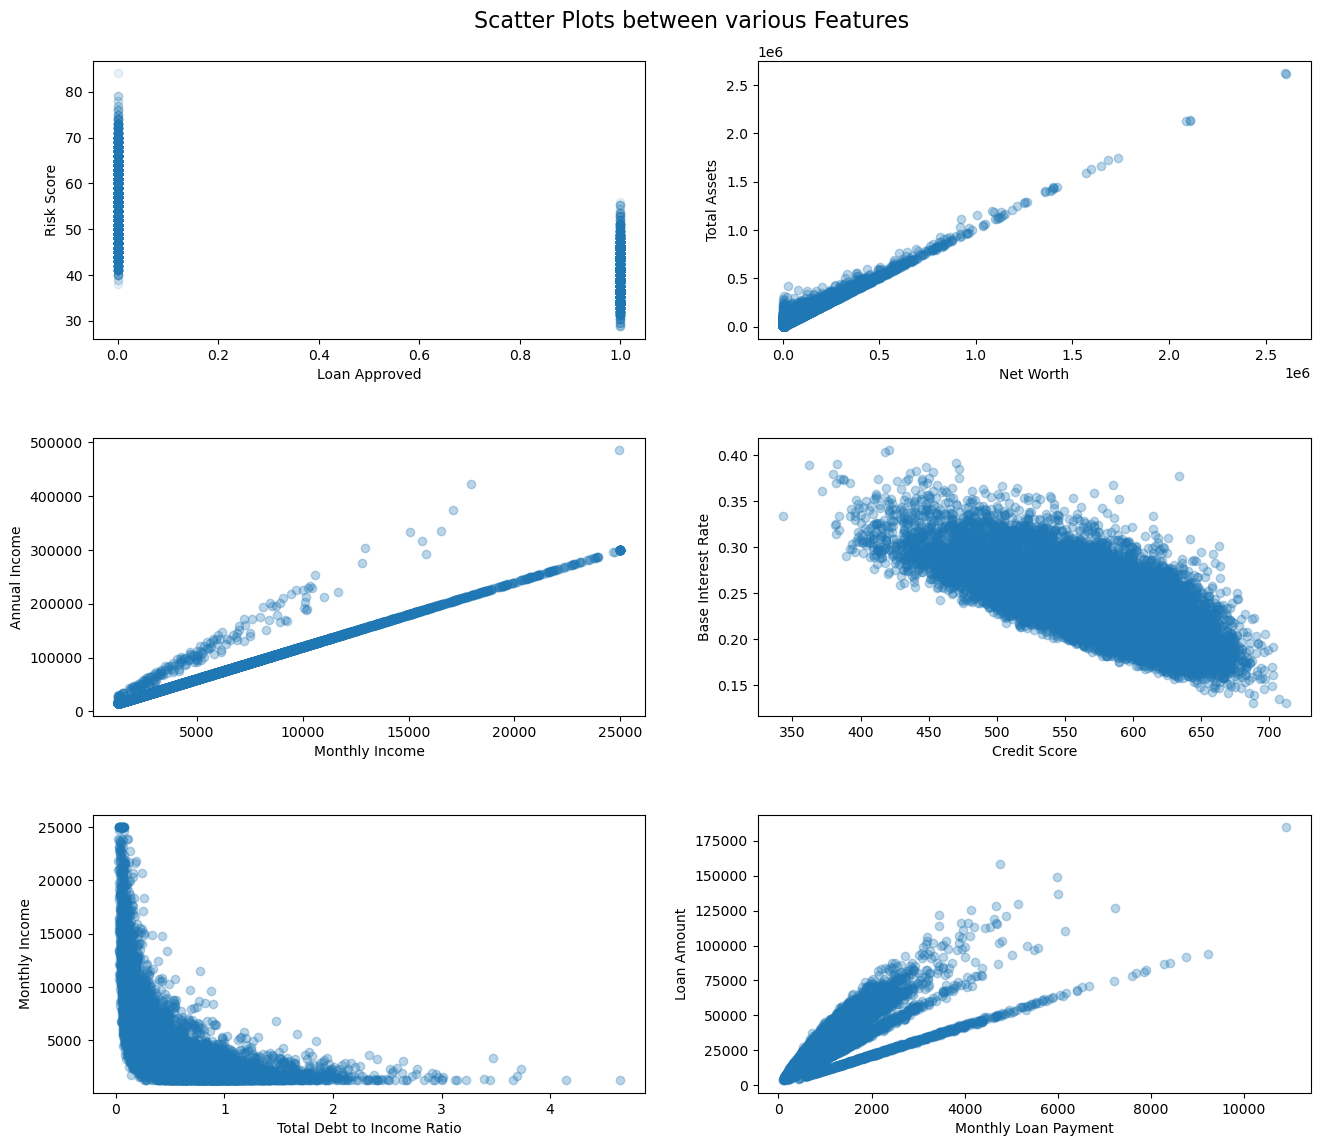
\includegraphics[width=0.9\paperwidth]{CorrScatters.png}}
\vspace*{\fill}

\newpage
\null
\vspace*{\fill}
\noindent\makebox[\textwidth]{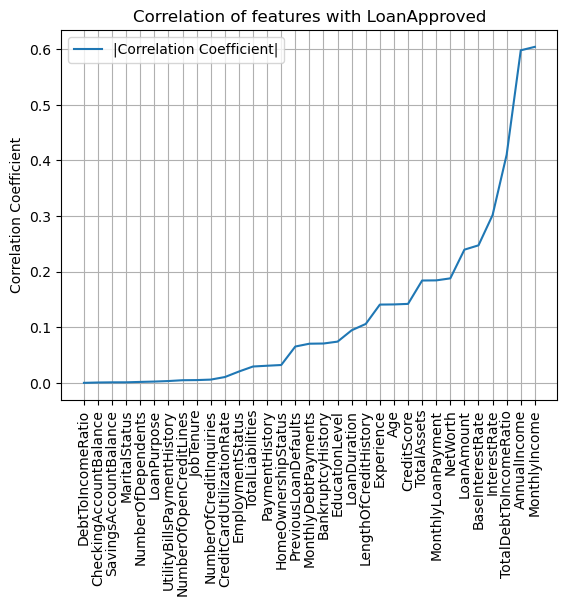
\includegraphics[width=0.8\paperwidth]{CorrWithLoanApproved.png}}
\vspace*{\fill}

\newpage
\null
\vspace*{\fill}
\noindent\makebox[\textwidth]{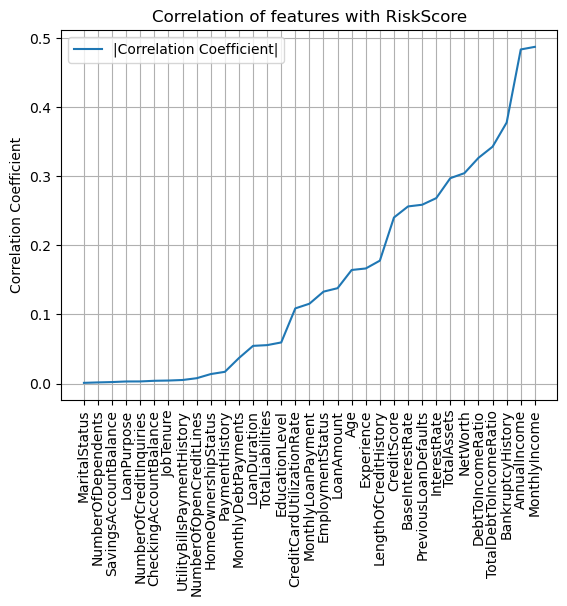
\includegraphics[width=0.8\paperwidth]{CorrWithRiskScore.png}}
\vspace*{\fill}

\newpage
\phantomsection
\addcontentsline{toc}{subsection}{Train-Validation-Test Split}
\noindent\textbf{Train-Validation-Test Split:}
We used a 60-20-20 split which resulted in a training set with 12000 examples and validation and test sets with 4000 examples each.
\\ \\

\phantomsection
\addcontentsline{toc}{subsection}{Outlier Processing}
\noindent\textbf{Outlier Processing:}
The \hyperref[boxplot]{\underline{boxplot}} shows presence of many outliers in the data. However, these cannot be simply removed or altered since they are valid data points. Hence we proceed with the data as it is.
\\ \\

\phantomsection
\addcontentsline{toc}{subsection}{Data Scaling}
\noindent\textbf{Data Scaling:}
Data has been processed through min-max scaling, Z-score scaling, and \href{https://scikit-learn.org/stable/modules/generated/sklearn.preprocessing.RobustScaler.html}{Robust Scaling (to deal with outliers)} separately.
\\ \\

\phantomsection
\addcontentsline{toc}{subsection}{Dimensional Reduction}
\noindent\textbf{Dimensional Reduction:}
The column \texttt{ApplicationDate} was dropped since it does not affect \texttt{LoanApproved} or \texttt{RiskScore}. Principal Component Analysis has been used to further reduce the dimensions of the data.

For data with integer labels, dimensions have been reduced from 33 to 10, 15, 20, and 25. For data with one-hot encoding, dimensions have been reduced from 49 to 15, 20, 25, 30, and 35.

\newpage
\noindent\makebox[\textwidth]{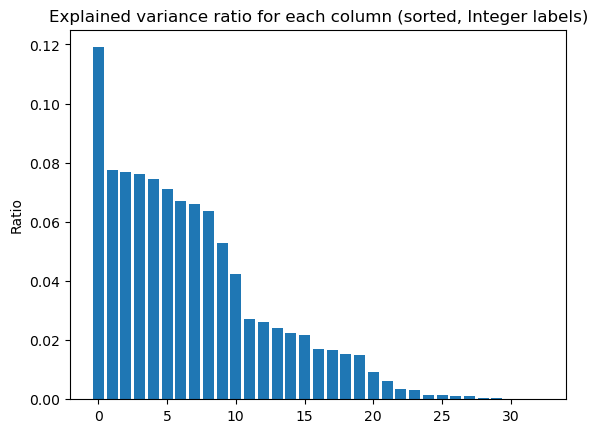
\includegraphics[width=0.9\paperwidth]{VarianceInt.png}}
\noindent\makebox[\textwidth]{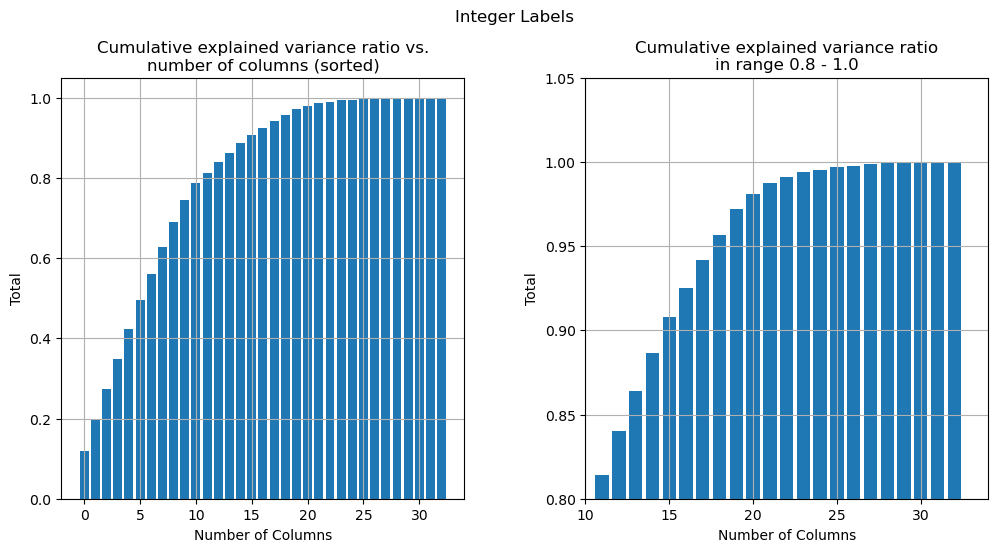
\includegraphics[width=0.9\paperwidth]{CumVarInt.png}}
\noindent\makebox[\textwidth]{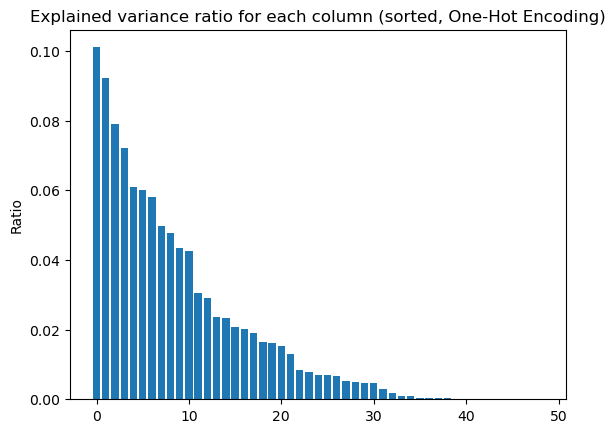
\includegraphics[width=0.9\paperwidth]{VarianceOH.png}}
\noindent\makebox[\textwidth]{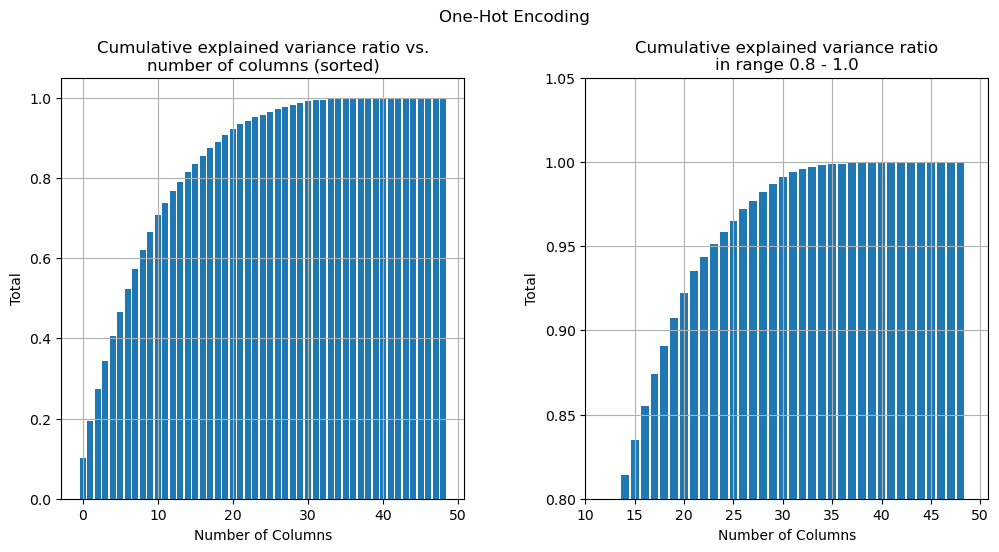
\includegraphics[width=0.9\paperwidth]{CumVarOH.png}}

\newpage
\chapter{Classification}
% \addcontentsline{toc}{chapter}{Classification}
The target variable \texttt{LoanApproved} is the second last column in the preprocessed datasets. We use the following models for classifying whether a loan request is approved or not:
\begin{itemize}
    \item $k$-Nearest Neighbors
    \item Logistic Regression
    \item Support Vector Machine
    \item Artificial Neural Networks
\end{itemize}

\section*{$k$-Nearest Neighbors}
\addcontentsline{toc}{section}{$k$-Nearest Neighbors}

\end{document}
